\section{Axis 1: Interface-Format Brittleness Is Trainably Fixable}
\label{sec:axis1}

The first axis is the simplest and the easiest to confuse for a
planner-quality effect.  Wrapping a GSM8K question in any
plan-shaped scaffold --- even an empty one --- moves \LLaDA{}'s
zero-shot accuracy.  This section measures the base hierarchy,
trains a small prefix-robust LoRA against it, and reports a
capacity tradeoff that exposes the axis as separable from sampling
diversity.

\subsection{The Base Hierarchy}
\label{subsec:axis1_hierarchy}

Table~\ref{tab:axis1_base_hierarchy} reports base
\LLaDA{}-8B-Instruct accuracy on GSM8K-test ($N{=}200$, $k{=}64$,
seed $0$) under five prefix conditions.

\begin{table}[h]
\centering
\caption{Base \LLaDA{} prefix-damage hierarchy on GSM8K-test, no
LoRA.  An empty \code{"Plan: "} prefix already costs $8$\,pp;
content-rich plans cost more, with the smaller \Qwen{1.5B} planner
producing the worst single-shot result.  The damage tracks prefix
shape, not plan quality.}
\label{tab:axis1_base_hierarchy}
\smallskip
\begin{tabular}{lr}
\toprule
Condition & Accuracy \\
\midrule
\ctwo{} (no prefix) & $\mathbf{74\%}$ \\
\code{C2hint} (\code{"Let's think step by step."}) & $68\%$ \\
\code{C2empty} (\code{"Plan: "}, no content) & $66\%$ \\
\cthree{}\code{p Q-0.5B} (weak plan) & $64\%$ \\
\cthree{}\code{p Q-1.5B} (medium plan) & $60\%$ \\
\bottomrule
\end{tabular}
\smallskip\\
{\footnotesize\textit{$95\%$ CIs (Clopper--Pearson, $N{=}200$):}
\ctwo{} \mbox{$[67.3, 79.9]$};
\code{C2hint} \mbox{$[61.1, 74.4]$};
\code{C2empty} \mbox{$[59.0, 72.5]$};
\cthree{}\code{p Q-0.5B} \mbox{$[56.9, 70.6]$};
\cthree{}\code{p Q-1.5B} \mbox{$[52.9, 66.8]$}.}
\end{table}

The empty-prefix \code{"Plan: "} condition costs $8$\,pp versus
no-prefix.  \LLaDA{}-8B-Instruct was not trained to ignore
plan-shaped scaffolds, and the literal token sequence --- not the
content --- is enough to perturb its reasoning.  This is the
single observation that motivated the present paper.

\subsection{Track 1 v2: A Small LoRA Flattens Static-Prefix Damage}
\label{subsec:axis1_v2}

We train a small LoRA on the prefix-robust dataset described in
\S\ref{sec:setup}.  v2 uses target modules
$[$\code{q\_proj}, \code{k\_proj}, \code{v\_proj}, \code{o\_proj},
\code{gate\_proj}, \code{up\_proj}, \code{down\_proj}$]$, the
standard Llama list.  Only $4$ of these module names match
\LLaDA{}'s actual block (\code{q\_proj}, \code{k\_proj},
\code{v\_proj}, \code{up\_proj}); the other three names are
absent from \LLaDA{}'s \code{LLaDALlamaBlock}.  The LoRA therefore
attaches to $4$ of $7$ intended modules and trains $\approx 10$M
parameters.  Hyperparameters: $r{=}8$, $\alpha{=}16$, learning rate
$5\mathrm{e}{-}5$, $5{,}000$ steps, $p_\text{mask} \sim U(0.1, 0.5)$.

Table~\ref{tab:axis1_v2_full} reports v2 against base on the full
prefix suite plus \code{cmaj b=5} ($t{=}0.7$).

\begin{table}[h]
\centering
\caption{Track 1 v2 versus base on GSM8K-test, $N{=}200$.  Static
prefix damage flattens (spread across \{\ctwo{}, \code{C2hint},
\code{C2empty}\} drops from $8$\,pp to $3$\,pp).  Q-1.5B plan
helps; Q-0.5B plan still hurts.  \cmaj{} accuracy is preserved on
dev.}
\label{tab:axis1_v2_full}
\smallskip
\begin{tabular}{lrrr}
\toprule
Condition & Base & v2 & $\Delta$ \\
\midrule
\ctwo{} & $74\%$ & $70.5\%$ & $-3.5$ \\
\code{C2hint} & $68\%$ & $73.5\%$ & $\mathbf{+5.5}$ \\
\code{C2empty} & $66\%$ & $73.0\%$ & $\mathbf{+7.0}$ \\
\cthree{}\code{p Q-0.5B} & $64\%$ & $60.0\%$ & $-4.0$ \\
\cthree{}\code{p Q-1.5B} & $60\%$ & $67.0\%$ & $\mathbf{+7.0}$ \\
\code{cmaj b=5} (dev) & $80\%$ & $81.5\%$ & $+1.5$ \\
\bottomrule
\end{tabular}
\smallskip\\
{\footnotesize\textit{$95\%$ CIs for v2 (Clopper--Pearson, $N{=}200$):}
\ctwo{} \mbox{$[63.7, 76.7]$};
\code{C2hint} \mbox{$[66.8, 79.5]$};
\code{C2empty} \mbox{$[66.3, 79.0]$};
\cthree{}\code{p Q-0.5B} \mbox{$[52.9, 66.8]$};
\cthree{}\code{p Q-1.5B} \mbox{$[60.0, 73.5]$};
\cmaj{} $b{=}5$ (dev) \mbox{$[75.4, 86.6]$}.}
\end{table}

The static-prefix spread \{\ctwo{}, \code{C2hint}, \code{C2empty}\}
collapses from $8$\,pp ($74 \to 66$) to $3$\,pp ($70.5 \to 73.5$).
The trained \cmaj{} branch-vote ceiling is preserved at $81.5\%$
on dev200.  No-prefix \ctwo{} loses $3.5$\,pp; we discuss this
tradeoff in the next subsection.  The Q-0.5B planner condition
still regresses ($64 \to 60$), and the Q-1.5B planner improves
($60 \to 67$): this directional split is the seed for the
planner-content-trust axis (\S\ref{sec:axis2}).

\subsection{Track 1 v3: A Capacity Tradeoff}
\label{subsec:axis1_v3}

While debugging Track 2 (the commit adapter,
\S\ref{sec:distill}), we discovered that \LLaDA{}'s
\code{LLaDALlamaBlock} uses olmo-style FFN names
(\code{ff\_proj}, \code{up\_proj}, \code{ff\_out}) instead of the
standard Llama \code{(gate\_proj, up\_proj, down\_proj)}.  v2's
target list matched only $4$ of $7$ intended modules.  v3 retrains
on the same data and hyperparameters with the \LLaDA{}-correct list
$[$\code{q\_proj}, \code{k\_proj}, \code{v\_proj}, \code{attn\_out},
\code{ff\_proj}, \code{up\_proj}, \code{ff\_out}$]$ --- a $7/7$
match, with $\approx 22$M trainable parameters ($2.2\times$ v2).

Table~\ref{tab:axis1_v2_v3} reports v2 against v3 on the same eval.

\begin{table}[h]
\centering
\caption{Track 1 v2 ($4/7$ modules, $10$M params) against v3 ($7/7$
modules, $22$M params) on GSM8K-test, $N{=}200$.  Full-FFN
coverage gains $+2.5$\,pp on no-prefix \ctwo{} but loses $-2.0$\,pp
on \cmaj{} branch-vote.  The Q-0.5B/Q-1.5B planner split
\emph{inverts} between the two capacities.  \cmaj{} on test for
v3 is reported apples-to-apples against base test \cmaj{} of
$79.0\%$.}
\label{tab:axis1_v2_v3}
\smallskip
\begin{tabular}{lrrrr}
\toprule
Condition & Base & v2 ($4/7$) & v3 ($7/7$) & v2$\to$v3 \\
\midrule
\ctwo{} & $74\%$ & $70.5\%$ & $\mathbf{73.0\%}$ & $+2.5$ \\
\code{C2hint} & $68\%$ & $73.5\%$ & $73.5\%$ & $0.0$ \\
\code{C2empty} & $66\%$ & $73.0\%$ & $74.0\%$ & $+1.0$ \\
\cthree{}\code{p Q-0.5B} & $64\%$ & $60.0\%$ & $\mathbf{65.0\%}$ & $+5.0$ \\
\cthree{}\code{p Q-1.5B} & $60\%$ & $67.0\%$ & $\mathbf{54.0\%}$ & $\mathbf{-13.0}$ \\
\code{cmaj b=5} & $79\%$ test, $80\%$ dev & $81.5\%$ (dev) & $79.5\%$ (test) & $-2.0$ \\
\bottomrule
\end{tabular}
\smallskip\\
{\footnotesize\textit{$95\%$ CIs for v3 (Clopper--Pearson, $N{=}200$):}
\ctwo{} \mbox{$[66.3, 79.0]$};
\code{C2hint} \mbox{$[66.8, 79.5]$};
\code{C2empty} \mbox{$[67.3, 79.9]$};
\cthree{}\code{p Q-0.5B} \mbox{$[58.0, 71.6]$};
\cthree{}\code{p Q-1.5B} \mbox{$[46.8, 61.1]$};
\cmaj{} $b{=}5$ (test) \mbox{$[73.2, 84.9]$}.  v2 column CIs are
listed under Table~\ref{tab:axis1_v2_full}; base column CIs under
Table~\ref{tab:axis1_base_hierarchy}.}
\end{table}

\begin{figure}[t]
\centering
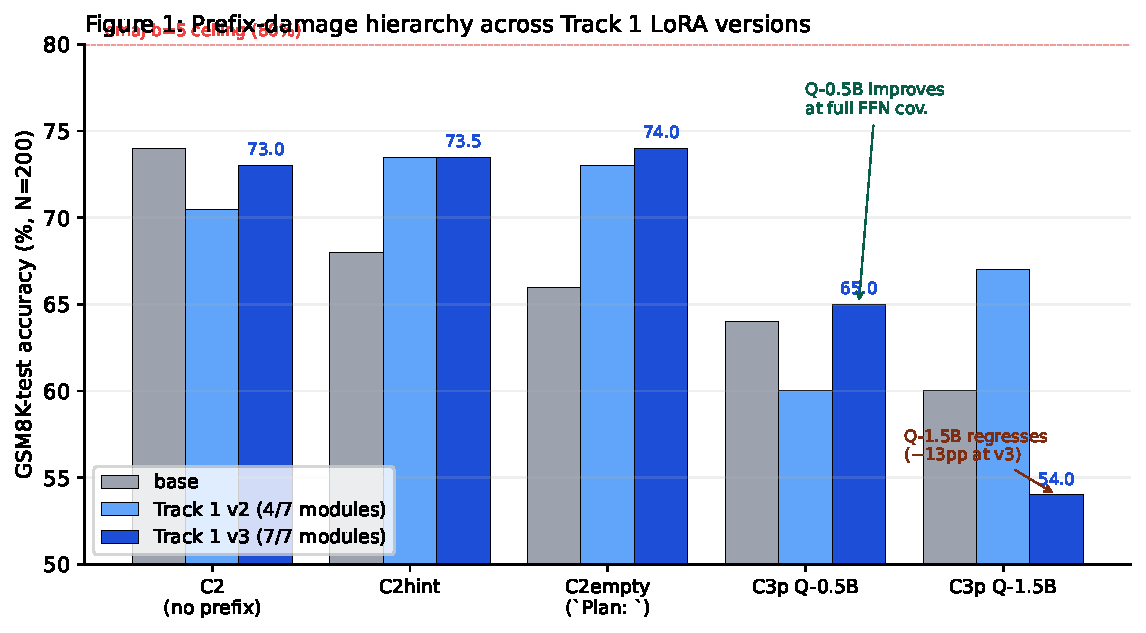
\includegraphics[width=\textwidth]{figures/fig1_prefix_hierarchy.pdf}
\caption{Prefix-damage hierarchy across \{base, Track 1 v2, Track
1 v3\} on all five conditions.  The \Qwen{0.5B}/\Qwen{1.5B}
inversion at v3 is annotated.  Static-prefix damage flattens at v2
and tightens further at v3; planner-content sensitivity widens at
v3.}
\label{fig:prefix_hierarchy}
\end{figure}

Two findings emerge from the v2-vs-v3 comparison.

\textbf{(a) A no-prefix-vs-\cmaj{} capacity tradeoff.}  Going from
$4/7$ to $7/7$ modules gains $+2.5$\,pp on no-prefix \ctwo{} but
loses $-2.0$\,pp on \cmaj{}.  Trainable parameters rise $10$M $\to$
$22$M ($2.2\times$).  Format-robustness on the static-prefix axis
and sampling-diversity-on-vote on the branch-vote axis are both
affected by Track-1-style training, but in opposite directions at
higher capacity.  We interpret this as additional capacity drifting
the model further from base on the high-confidence answer-token
path that vote-aggregation relies on; the \cmaj{} ensemble is more
sensitive to per-branch drift than the single-shot reading is.

\textbf{(b) The planner-quality split inverts.}  At v2 capacity
the bigger \Qwen{1.5B} planner produces better plans and the
adapter uses them ($+7$\,pp).  At v3 capacity, the same bigger
planner causes a $-13$\,pp regression while the smaller
\Qwen{0.5B} planner improves $+5$\,pp.  This is the seed for
\S\ref{sec:axis2}: capacity does not just flatten format
brittleness, it modulates content trust, and the direction of the
effect is opposite for the two planners.

\subsection{Reading}
\label{subsec:axis1_reading}

Track 1 establishes that interface-format brittleness is a real,
isolable, trainable axis.  An $r{=}8$ LoRA on a small
prefix-randomized dataset closes the static-prefix damage gap from
$8$\,pp to within $1$\,pp at v3 capacity.  The cost is split
between $-2.0$\,pp on \cmaj{} (capacity tradeoff) and a widened
spread across content-rich plans (motivating \S\ref{sec:axis2}).
For deployment, the v2-vs-v3 choice depends on whether the
downstream pipeline uses single-shot (v3 wins by $+2.5$\,pp on
\ctwo{}) or branch-vote (v2 wins by $+2.0$\,pp on \cmaj{}).

\paragraph{Status.}
Track 1's prefix-robustness fix is robust on GSM8K-test
$N{=}200$, single seed, with the prefix-tier distribution
described in \S\ref{sec:setup}.  Cross-task transfer (e.g.\
MATH-Easy, ARC-Challenge) and multi-seed variance are open and
flagged in \appref{app:open}; both are cheap follow-ups that
would harden the headline numbers without changing the framing.
